%*******10********20********30********40********50********60********70********80
\clearpage
\subsection{Expansion Ratio Related to Behavior of Concrete During ASR Expansion}

In this section, the relationship between given initial strain, final expansion and behavior during expansion is discussed.

Model in size of $100 \times 100 \times 100$ mm is in used (Figure \ref{ASRRRR}), with 30\% Aggregate (75\% of which is ASR reactive).

\begin{figure}[ht]
\centering
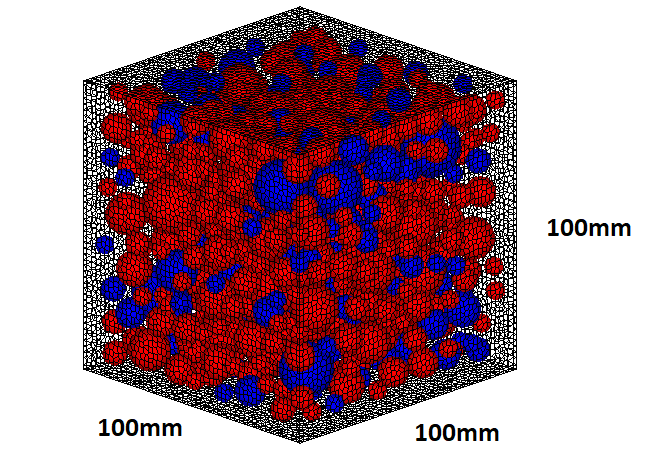
\includegraphics[width=.3\linewidth]{Files/Aggregate/A30P75.png}
  \caption{30\% Coarse Aggregate}
  \label{ASRRRR}
\end{figure}

Expansion is carried out with initial strain given in each step various from 0 to 0.003. Total expansion step are set as 20 steps same for all cases. From the Table \ref{table:ASR_30_EXPppp} can be seen that with the increasing of giving initial strain in each step, the global expansion reached in step 20 also increased. Non-damage model is using here for compare.

\begin{table}[ht!]

\caption{One Dimensional Expansion Ratio in Single ASR Model Simulation}

\centering
\begin{tabular}{ ||p{2cm}|p{2cm}|p{2cm}|p{2cm}|p{2cm}|| }
 \hline
 Aggregate Ratio[\%] &  Reactive Aggregate Ratio[\%]  & Initial Strain (Each Step) & Expanding Steps & Final Expansion [\%] \\ [0.5ex]
 \hline\hline
 30 & 75 & 0 & 0 & 0\\
 30 & 75 & 0.0002 & 20 & 0.0699\\
 30 & 75 & 0.0005 & 20 & 0.1936\\
 30 & 75 & 0.001 & 20 & 0.4223\\
 30 & 75 & 0.002 & 20 & 0.8832\\
 30 & 75 & 0.003 & 20 & 1.3224\\
 \hline
\end{tabular}

\label{table:ASR_30_EXPppp}
\end{table}

\begin{figure}[!h]
\centering

    %*******
    \begin{subfigure}{.5\textwidth}
      \centering
      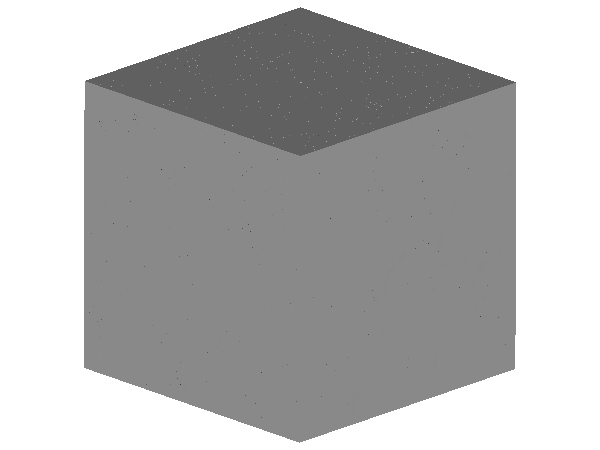
\includegraphics[width=.8\linewidth]{Files/exp_3D/ASR/A30Undamaged.png}
    \caption{Case 0: 0\% Expansion}
    \end{subfigure}%
    %*******
    \begin{subfigure}{.5\textwidth}
      \centering
      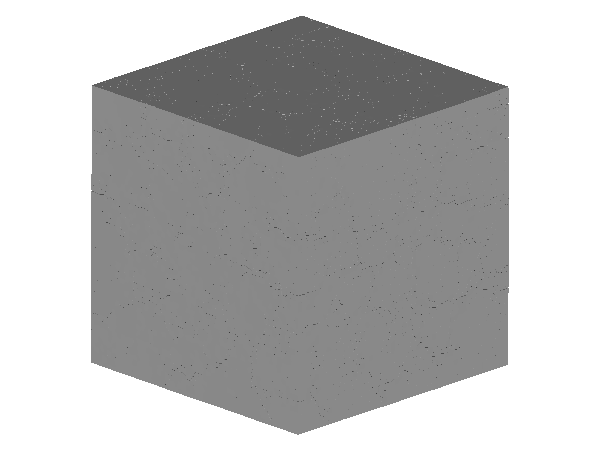
\includegraphics[width=.8\linewidth]{Files/exp_3D/ASR/A30P75_1_3d.png}
    \caption{Case 1: 0.0699\% Expansion}
    \end{subfigure}
    %*******
    \begin{subfigure}{.5\textwidth}
      \centering
      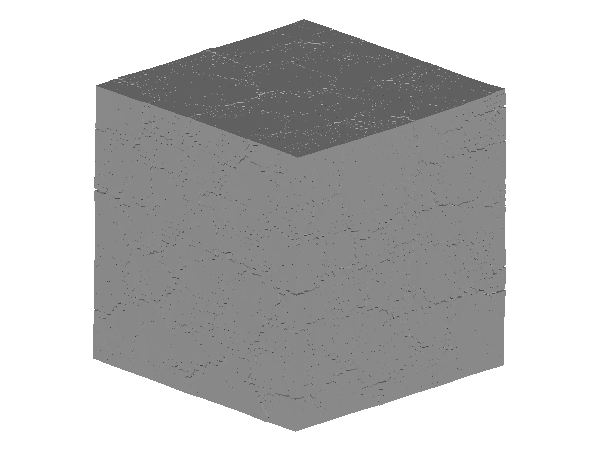
\includegraphics[width=.8\linewidth]{Files/exp_3D/ASR/A30P75_2_3d.png}
    \caption{Case 2: 0.1936\% Expansion}
    \end{subfigure}%
    %*******
    \begin{subfigure}{.5\textwidth}
      \centering
      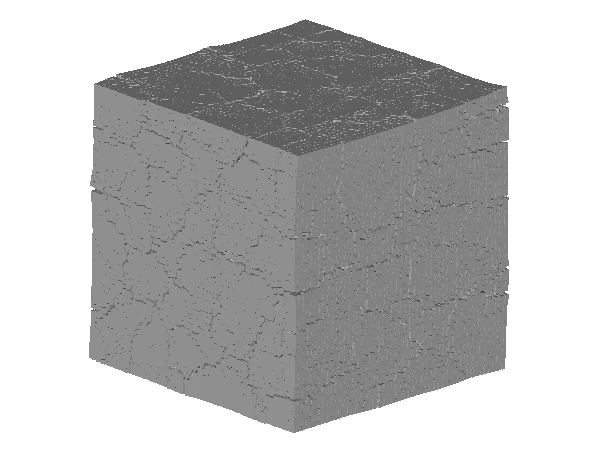
\includegraphics[width=.8\linewidth]{Files/exp_3D/ASR/A30P75_3_3d.png}
    \caption{Case 3: 0.4223\% Expansion}
    \end{subfigure}
    %*******
    \begin{subfigure}{.5\textwidth}
      \centering
      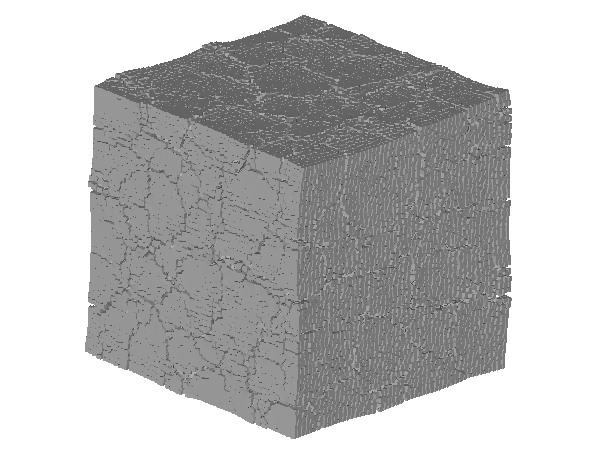
\includegraphics[width=.8\linewidth]{Files/exp_3D/ASR/A30P75_4_3d.png}
    \caption{Case 4: 0.8832\% Expansion}
    \end{subfigure}%
    %*******
    \begin{subfigure}{.5\textwidth}
      \centering
      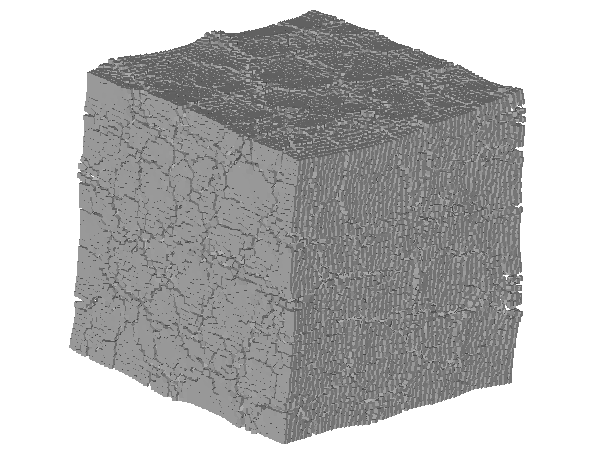
\includegraphics[width=.8\linewidth]{Files/exp_3D/ASR/A30P75_5_3d.png}
    \caption{Case 5: 1.3224\% Expansion}
    \end{subfigure}
    %*******

  \caption{3D Surface Cracks ($Deformation \times 10$)}
  \label{fig:ASR_A30P75_3D}
\end{figure}

% Surface of one side
\begin{figure}[!h]
\centering

    %*******
    \begin{subfigure}{.5\textwidth}
      \centering
      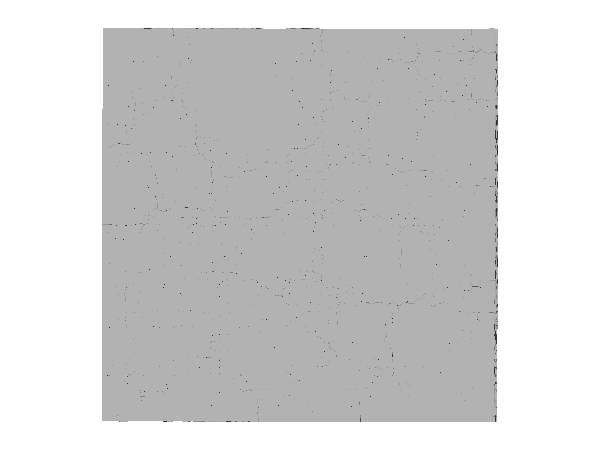
\includegraphics[width=.8\linewidth]{Files/exp_3D/ASR/A30P75_1_3ds.png}
    \caption{Case 0: 0\% Expansion}
    \end{subfigure}%
    %*******
    \begin{subfigure}{.5\textwidth}
      \centering
      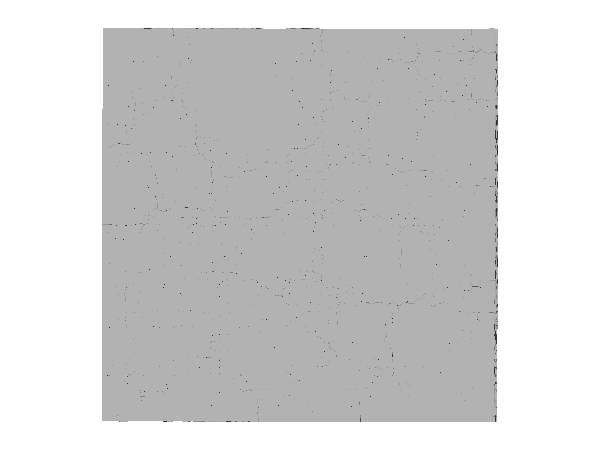
\includegraphics[width=.8\linewidth]{Files/exp_3D/ASR/A30P75_1_3ds.png}
    \caption{Case 1: 0.0699\% Expansion}
    \end{subfigure}
    %*******
    \begin{subfigure}{.5\textwidth}
      \centering
      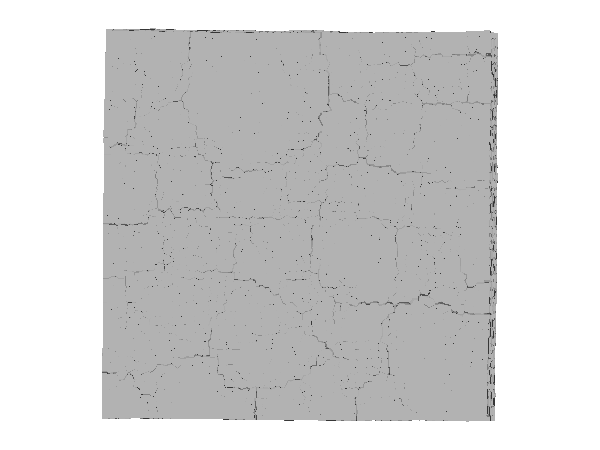
\includegraphics[width=.8\linewidth]{Files/exp_3D/ASR/A30P75_2_3ds.png}
    \caption{Case 2: 0.1936\% Expansion}
    \end{subfigure}%
    %*******
    \begin{subfigure}{.5\textwidth}
      \centering
      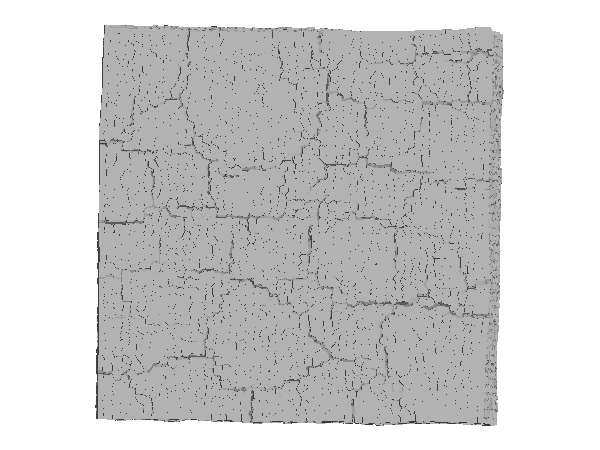
\includegraphics[width=.8\linewidth]{Files/exp_3D/ASR/A30P75_3_3ds.png}
    \caption{Case 3: 0.4223\% Expansion}
    \end{subfigure}
    %*******
    \begin{subfigure}{.5\textwidth}
      \centering
      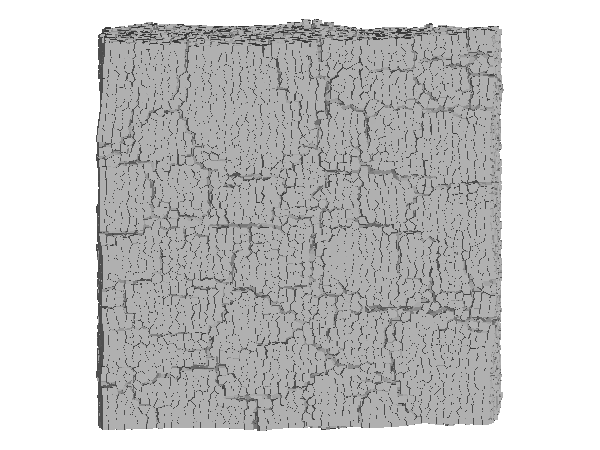
\includegraphics[width=.8\linewidth]{Files/exp_3D/ASR/A30P75_4_3ds.png}
    \caption{Case 4: 0.8832\% Expansion}
    \end{subfigure}%
    %*******
    \begin{subfigure}{.5\textwidth}
      \centering
      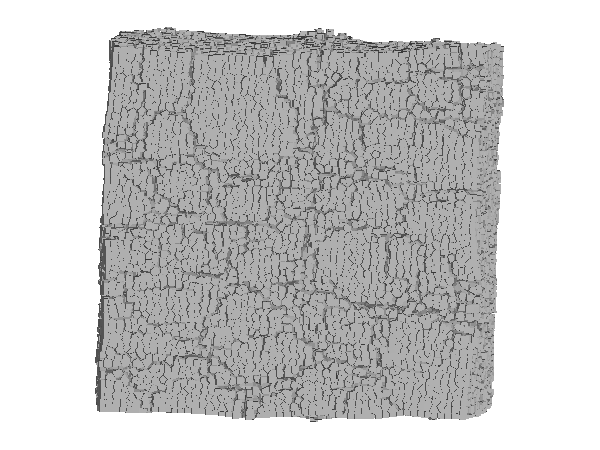
\includegraphics[width=.8\linewidth]{Files/exp_3D/ASR/A30P75_5_3ds.png}
    \caption{Case 5: 1.3224\% Expansion}
    \end{subfigure}
    %*******

  \caption{3D Surface Cracks (Single Side View, $Deformation \times 10$)}
  \label{fig:ASR_A30P75_3DS}
\end{figure}

As shown in Figure \ref{fig:ASR_A30P75_3D} and Figure \ref{fig:ASR_A30P75_3DS}, it is clear that with the increase of global expansion ratio, the cracking can be seen on the surface of concrete model become much significant. However, the map cracking pattern does not change much comparing the expanded models in different expansion ratio.

This also indicated that our simulation can still predict the map cracking behavior for ASR expansion in different deterioration levels.

It is possible that the position where large crack generated is determined by other factors, for example, the location of coarse aggregate.

\clearpage

\begin{figure}[!h]
\centering

    %*******
    \begin{subfigure}{.5\textwidth}
      \centering
      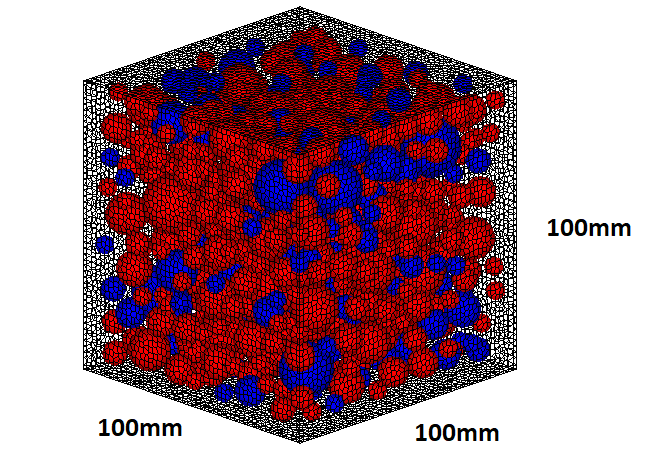
\includegraphics[width=.8\linewidth]{Files/Aggregate/A30P75.png}
    \caption{Case 0: 0\% Expansion}
    \end{subfigure}%
    %*******
    \begin{subfigure}{.5\textwidth}
      \centering
      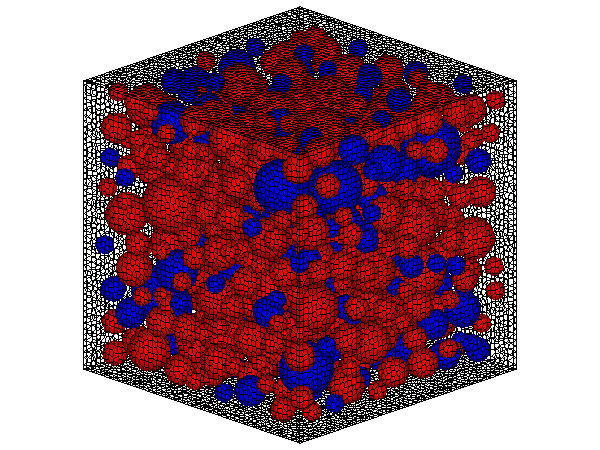
\includegraphics[width=.8\linewidth]{Files/exp_3D/ASR/A30P75_1_c.png}
    \caption{Case 1: 0.0699\% Expansion}
    \end{subfigure}
    %*******
    \begin{subfigure}{.5\textwidth}
      \centering
      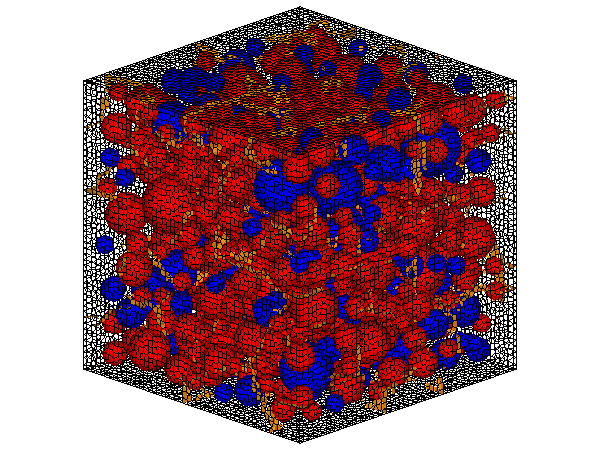
\includegraphics[width=.8\linewidth]{Files/exp_3D/ASR/A30P75_2_c.png}
    \caption{Case 2: 0.1936\% Expansion}
    \end{subfigure}%
    %*******
    \begin{subfigure}{.5\textwidth}
      \centering
      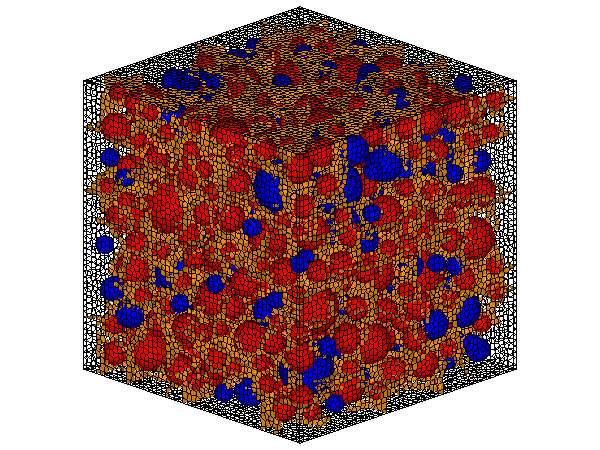
\includegraphics[width=.8\linewidth]{Files/exp_3D/ASR/A30P75_3_c.png}
    \caption{Case 3: 0.4223\% Expansion}
    \end{subfigure}
    %*******
    \begin{subfigure}{.5\textwidth}
      \centering
      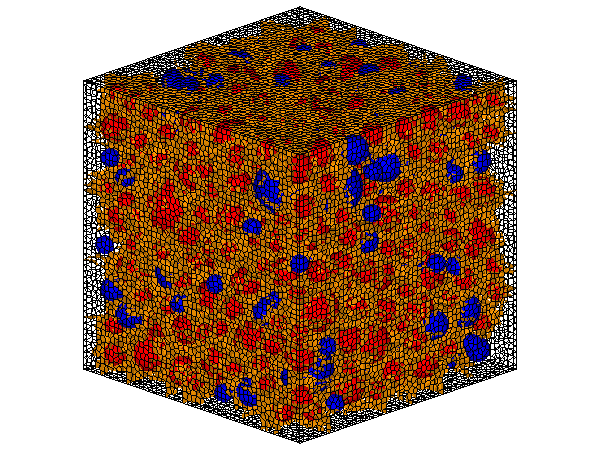
\includegraphics[width=.8\linewidth]{Files/exp_3D/ASR/A30P75_4_c.png}
    \caption{Case 4: 0.8832\% Expansion}
    \end{subfigure}%
    %*******
    \begin{subfigure}{.5\textwidth}
      \centering
      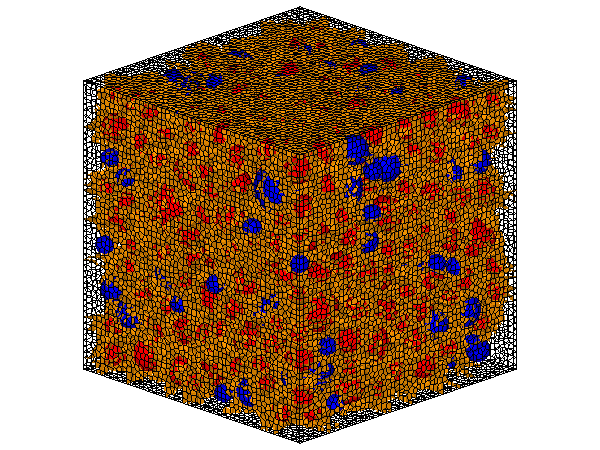
\includegraphics[width=.8\linewidth]{Files/exp_3D/ASR/A30P75_5_c.png}
    \caption{Case 5: 1.3224\% Expansion}
    \end{subfigure}
    %*******

  \caption{3D Inner Crack Width Larger than 0.03 mm}
  \label{fig:ASR_A30P75_crack}
\end{figure}

By comparing the inner cracking condition in Figure \ref{fig:ASR_A30P75_crack}, it can be seen that start from 0.1936\% of one-dimensional global expansion, cracks larger than 0.03 mm are generated and able to be recognizable by the naked eye. With the increase of global expansion ratio, the inner crack generally increases, distributed relatively uniform in all inner part of the expanded model. This cracking pattern will be compared with ASR expansion in different reactive aggregate ratio simulation and also DEF simulations.

%% ASR_A30_P75_3 Internal Stress
\begin{figure}[h!]
\centering
    %*******
    %*******
    \begin{subfigure}{.25\textwidth}
      \centering
      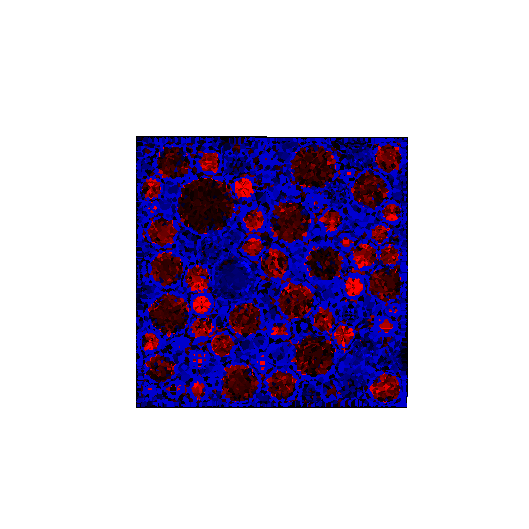
\includegraphics[width=1.0\linewidth]{Files/exp_3D/ASR/A30P75_1_s5.png}
      \caption{0.0699\% Expansion\\Internal Stress Step 5}
    \end{subfigure}%
    %*******
    \begin{subfigure}{.25\textwidth}
      \centering
      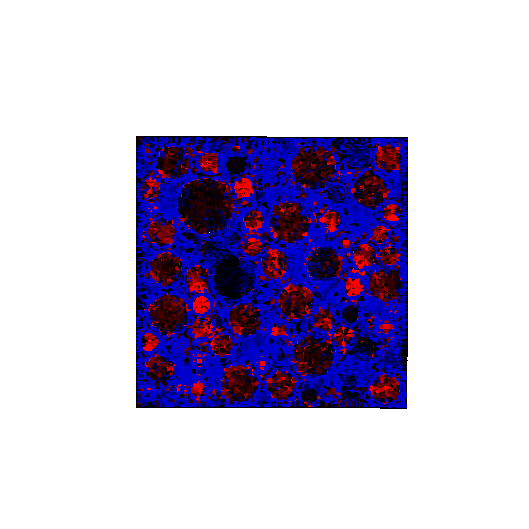
\includegraphics[width=1.0\linewidth]{Files/exp_3D/ASR/A30P75_1_s10.png}
      \caption{0.0699\% Expansion\\Internal Stress Step 10}
    \end{subfigure}%
    %*******
    \begin{subfigure}{.25\textwidth}
      \centering
      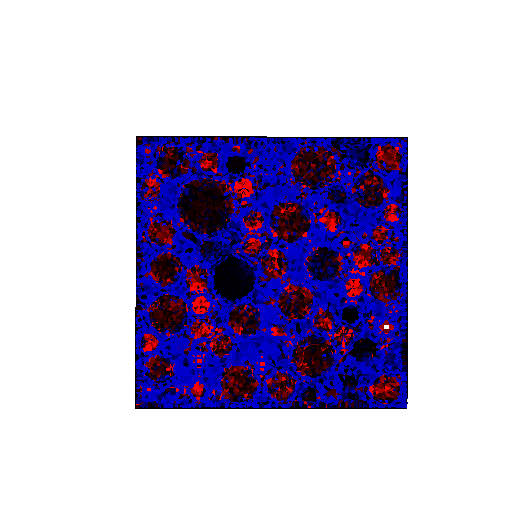
\includegraphics[width=1.0\linewidth]{Files/exp_3D/ASR/A30P75_1_s15.png}
      \caption{0.0699\% Expansion\\Internal Stress Step 15}
    \end{subfigure}%
    %*******
    \begin{subfigure}{.25\textwidth}
      \centering
      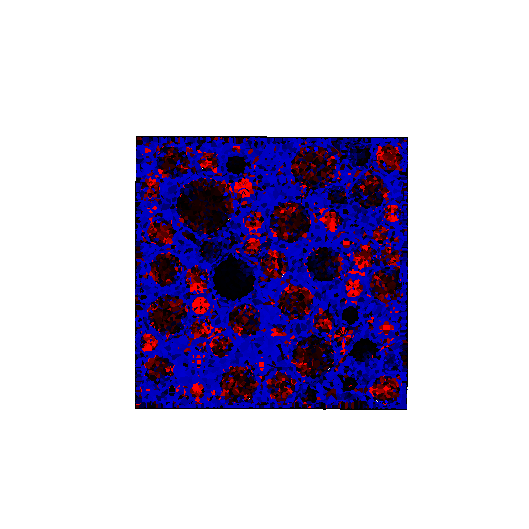
\includegraphics[width=1.0\linewidth]{Files/exp_3D/ASR/A30P75_1_stress.png}
      \caption{0.0699\% Expansion\\Internal Stress Step 20}
    \end{subfigure}
    %*******
    %*******
    \begin{subfigure}{.25\textwidth}
      \centering
      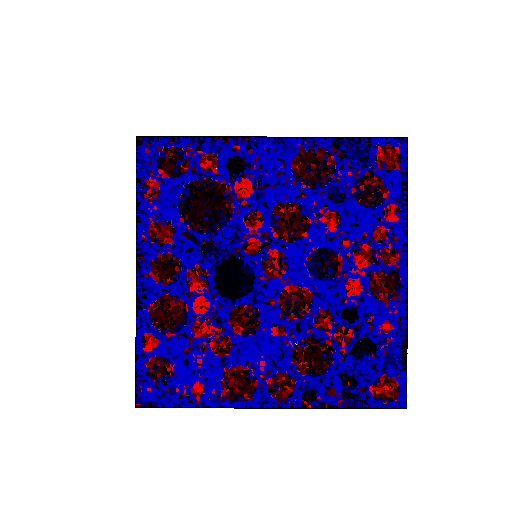
\includegraphics[width=1.0\linewidth]{Files/exp_3D/ASR/A30P75_2_s5.png}
      \caption{0.1936\% Expansion\\Internal Stress Step 5}
    \end{subfigure}%
    %*******
    \begin{subfigure}{.25\textwidth}
      \centering
      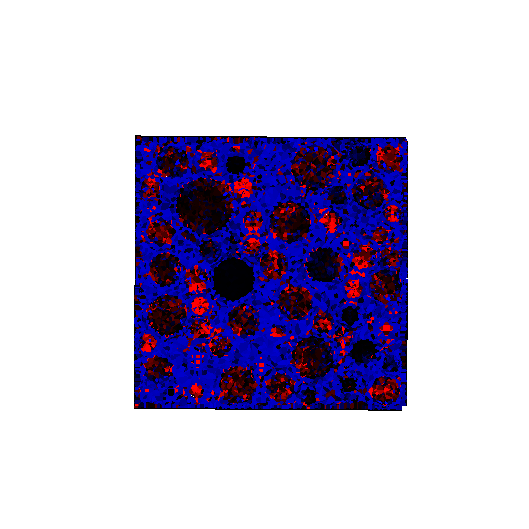
\includegraphics[width=1.0\linewidth]{Files/exp_3D/ASR/A30P75_2_s10.png}
      \caption{0.1936\% Expansion\\Internal Stress Step 10}
    \end{subfigure}%
    %*******
    \begin{subfigure}{.25\textwidth}
      \centering
      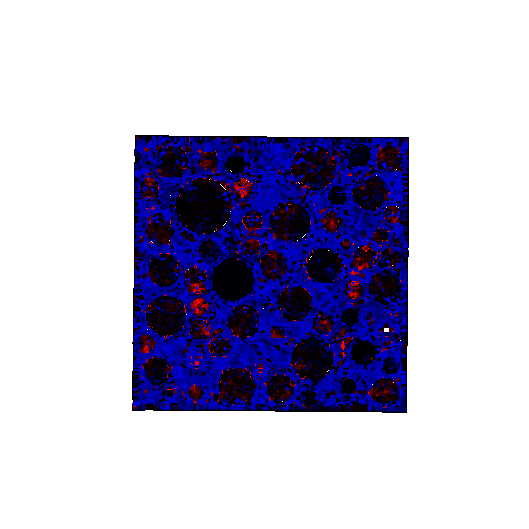
\includegraphics[width=1.0\linewidth]{Files/exp_3D/ASR/A30P75_2_s15.png}
      \caption{0.1936\% Expansion\\Internal Stress Step 15}
    \end{subfigure}%
    %*******
    \begin{subfigure}{.25\textwidth}
      \centering
      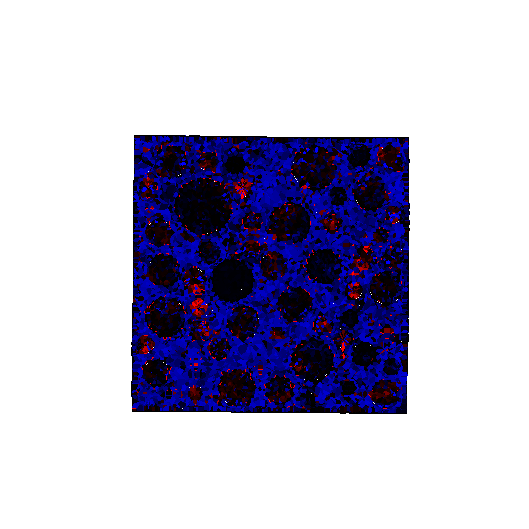
\includegraphics[width=1.0\linewidth]{Files/exp_3D/ASR/A30P75_2_stress.png}
      \caption{0.1936\% Expansion\\Internal Stress Step 20}
    \end{subfigure}
    %*******
    %*******
    \begin{subfigure}{.25\textwidth}
      \centering
      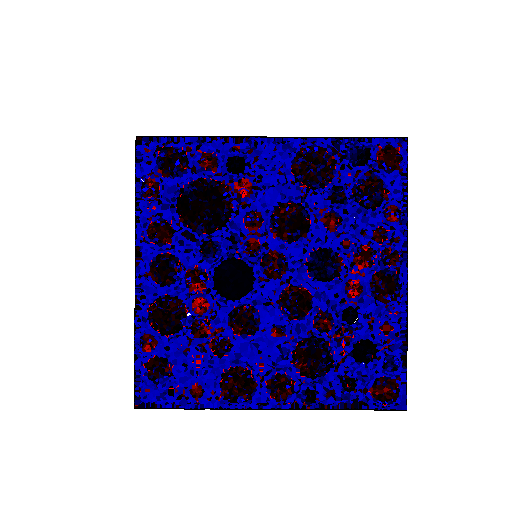
\includegraphics[width=1.0\linewidth]{Files/exp_3D/ASR/A30P75_3_s5.png}
      \caption{0.4223\% Expansion\\Internal Stress Step 5}
    \end{subfigure}%
    %*******
    \begin{subfigure}{.25\textwidth}
      \centering
      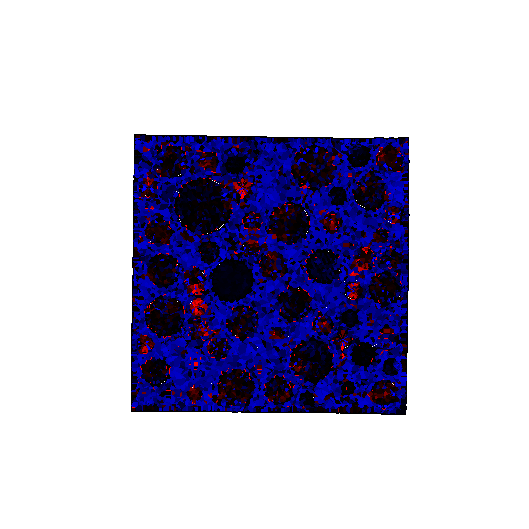
\includegraphics[width=1.0\linewidth]{Files/exp_3D/ASR/A30P75_3_s10.png}
      \caption{0.4223\% Expansion\\Internal Stress Step 10}
    \end{subfigure}%
    %*******
    \begin{subfigure}{.25\textwidth}
      \centering
      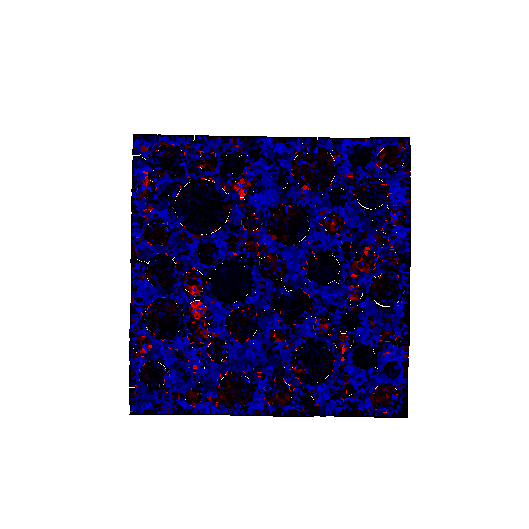
\includegraphics[width=1.0\linewidth]{Files/exp_3D/ASR/A30P75_3_s15.png}
      \caption{0.4223\% Expansion\\Internal Stress Step 15}
    \end{subfigure}%
    %*******
    \begin{subfigure}{.25\textwidth}
      \centering
      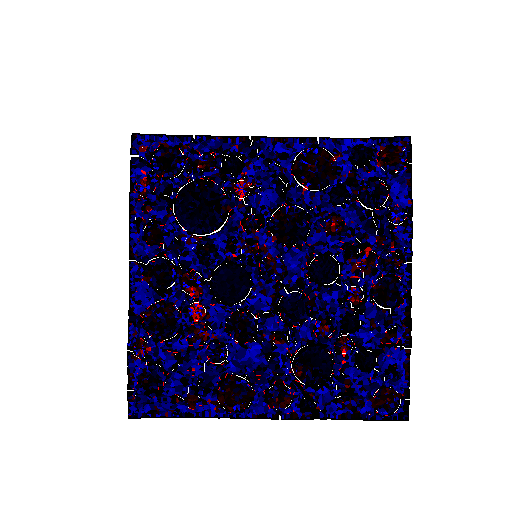
\includegraphics[width=1.0\linewidth]{Files/exp_3D/ASR/A30P75_3_stress.png}
      \caption{0.4223\% Expansion\\Internal Stress Step 20}
    \end{subfigure}
    %*******

    %*******
    \begin{subfigure}{.25\textwidth}
      \centering
      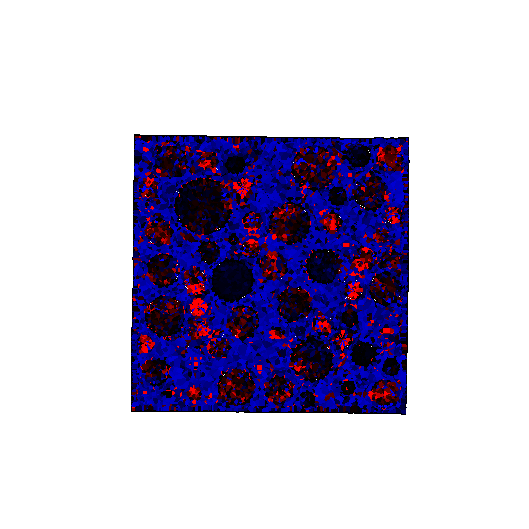
\includegraphics[width=1.0\linewidth]{Files/exp_3D/ASR/A30P75_4_s5.png}
      \caption{0.8832\% Expansion\\Internal Stress Step 5}
    \end{subfigure}%
    %*******
    \begin{subfigure}{.25\textwidth}
      \centering
      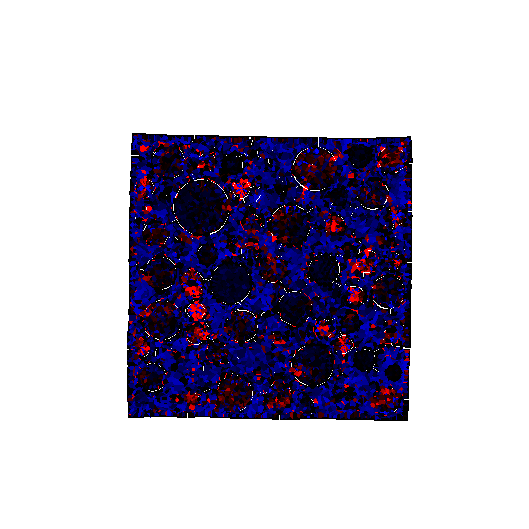
\includegraphics[width=1.0\linewidth]{Files/exp_3D/ASR/A30P75_4_s10.png}
      \caption{0.8832\% Expansion\\Internal Stress Step 10}
    \end{subfigure}%
    %*******
    \begin{subfigure}{.25\textwidth}
      \centering
      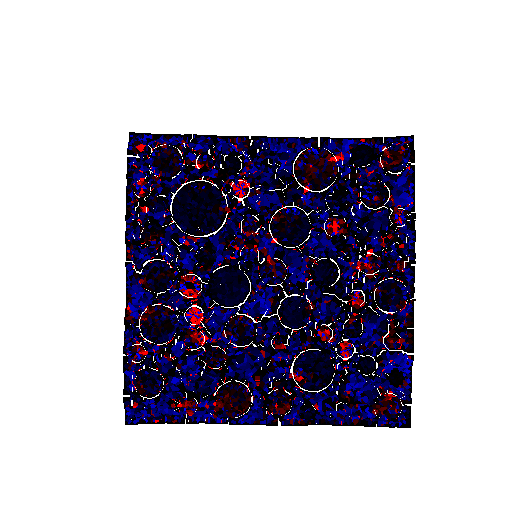
\includegraphics[width=1.0\linewidth]{Files/exp_3D/ASR/A30P75_4_s15.png}
      \caption{0.8832\% Expansion\\Internal Stress Step 15}
    \end{subfigure}%
    %*******
    \begin{subfigure}{.25\textwidth}
      \centering
      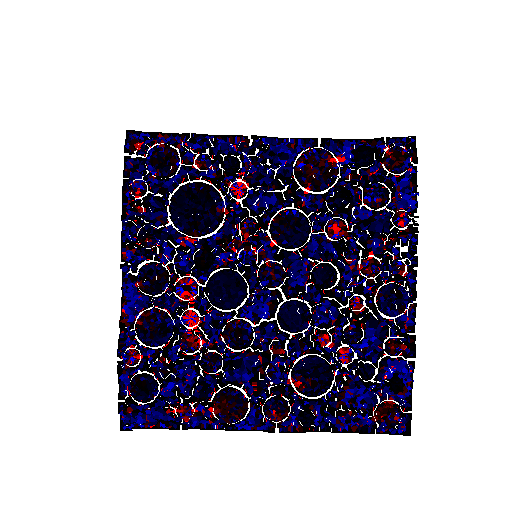
\includegraphics[width=1.0\linewidth]{Files/exp_3D/ASR/A30P75_4_stress.png}
      \caption{0.8832\% Expansion\\Internal Stress Step 20}
    \end{subfigure}
    %*******

    %*******
    \begin{subfigure}{.25\textwidth}
      \centering
      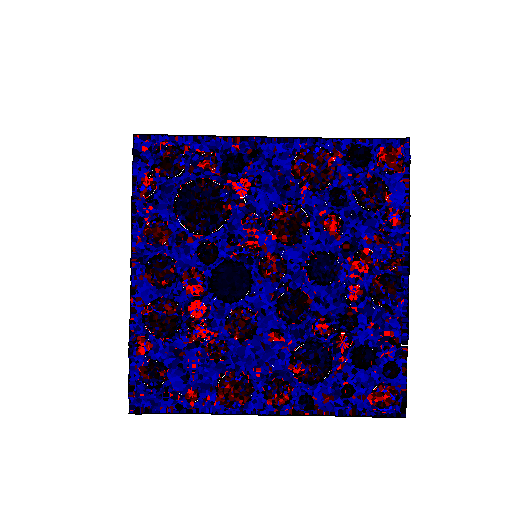
\includegraphics[width=1.0\linewidth]{Files/exp_3D/ASR/A30P75_5_s5.png}
      \caption{1.3224\% Expansion\\Internal Stress Step 5}
    \end{subfigure}%
    %*******
    \begin{subfigure}{.25\textwidth}
      \centering
      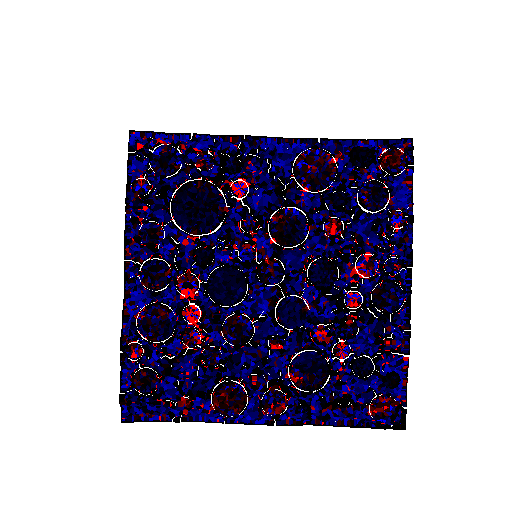
\includegraphics[width=1.0\linewidth]{Files/exp_3D/ASR/A30P75_5_s10.png}
      \caption{1.3224\% Expansion\\Internal Stress Step 10}
    \end{subfigure}%
    %*******
    \begin{subfigure}{.25\textwidth}
      \centering
      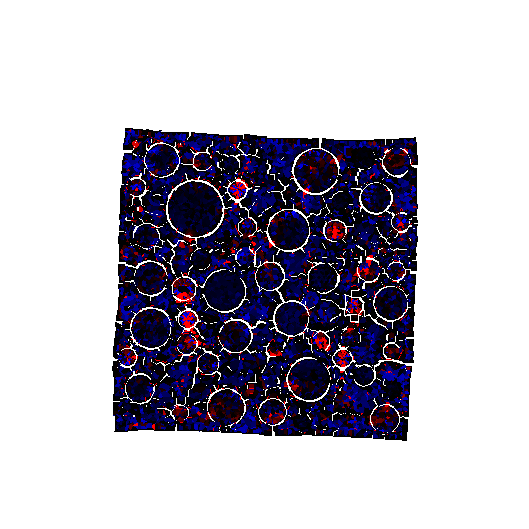
\includegraphics[width=1.0\linewidth]{Files/exp_3D/ASR/A30P75_5_s15.png}
      \caption{1.3224\% Expansion\\Internal Stress Step 15}
    \end{subfigure}%
    %*******
    \begin{subfigure}{.25\textwidth}
      \centering
      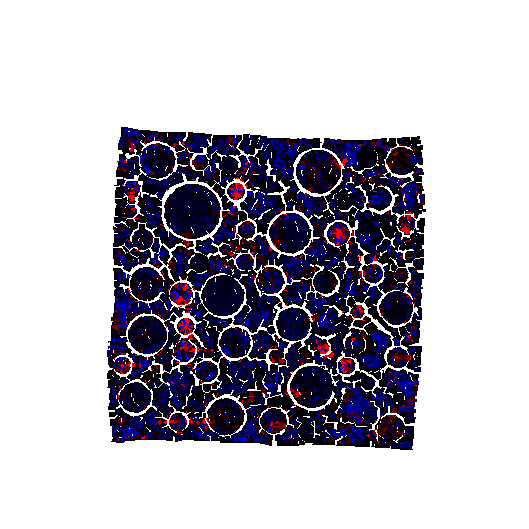
\includegraphics[width=1.0\linewidth]{Files/exp_3D/ASR/A30P75_5_stress.png}
      \caption{1.3224\% Expansion\\Internal Stress Step 20}
    \end{subfigure}
    %*******

    \begin{subfigure}{0.8\textwidth}
  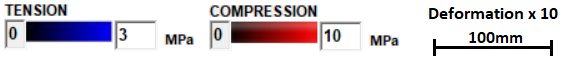
\includegraphics[width=0.8\linewidth]{Files/exp_3D/tagCS10.png}
\end{subfigure}%


\caption{Generation of Internal Stress and Inner Cracks for ASR Expansion[\%] to Step 20(Final Expansion Step, $Deformation \times 10$)}
\label{fig:A30_P75_stress}
\end{figure}

\clearpage

In Figure \ref{fig:A30_P75_stress}, the internal stress distribution in some middle step and last expansion step are shown. By increasing the initial strain giving to present ASR expansion in each step, the expansion developed more rapidly and more inner cracks generated as well as outer cracks.

This suggests deteration caused by ASR not only causing the aesthetic problem on the surface of the concrete structure but also indicate structually damage inside.

By visualizing the inner crack, we can confirm that the inner part of the ASR-damaged concrete model also deteriorated. As the increasing of global expansion, inner cracks gradually increase its number and volume, in cases over 0.8\% global expansion, crack with a width larger than 0.03 mm almost covered all inner part of the expanded model.

The advantage of 3D RBSM also allows us to obtain the precise number of cracked internal faces at the end of each expansion process. Here in Figure \ref{A30P75CRACKkk} the cracked interfaces in corresponding of expansion separated by crack width are presented.

It can be seen that with the increase of global expansion, cracks are all width range increase its number gradually. Larger cracks appear later during expansion comparing to cracks in a smaller width, which are easier to generate even with a very small global expansion.

\begin{figure}[ht!]
\centering
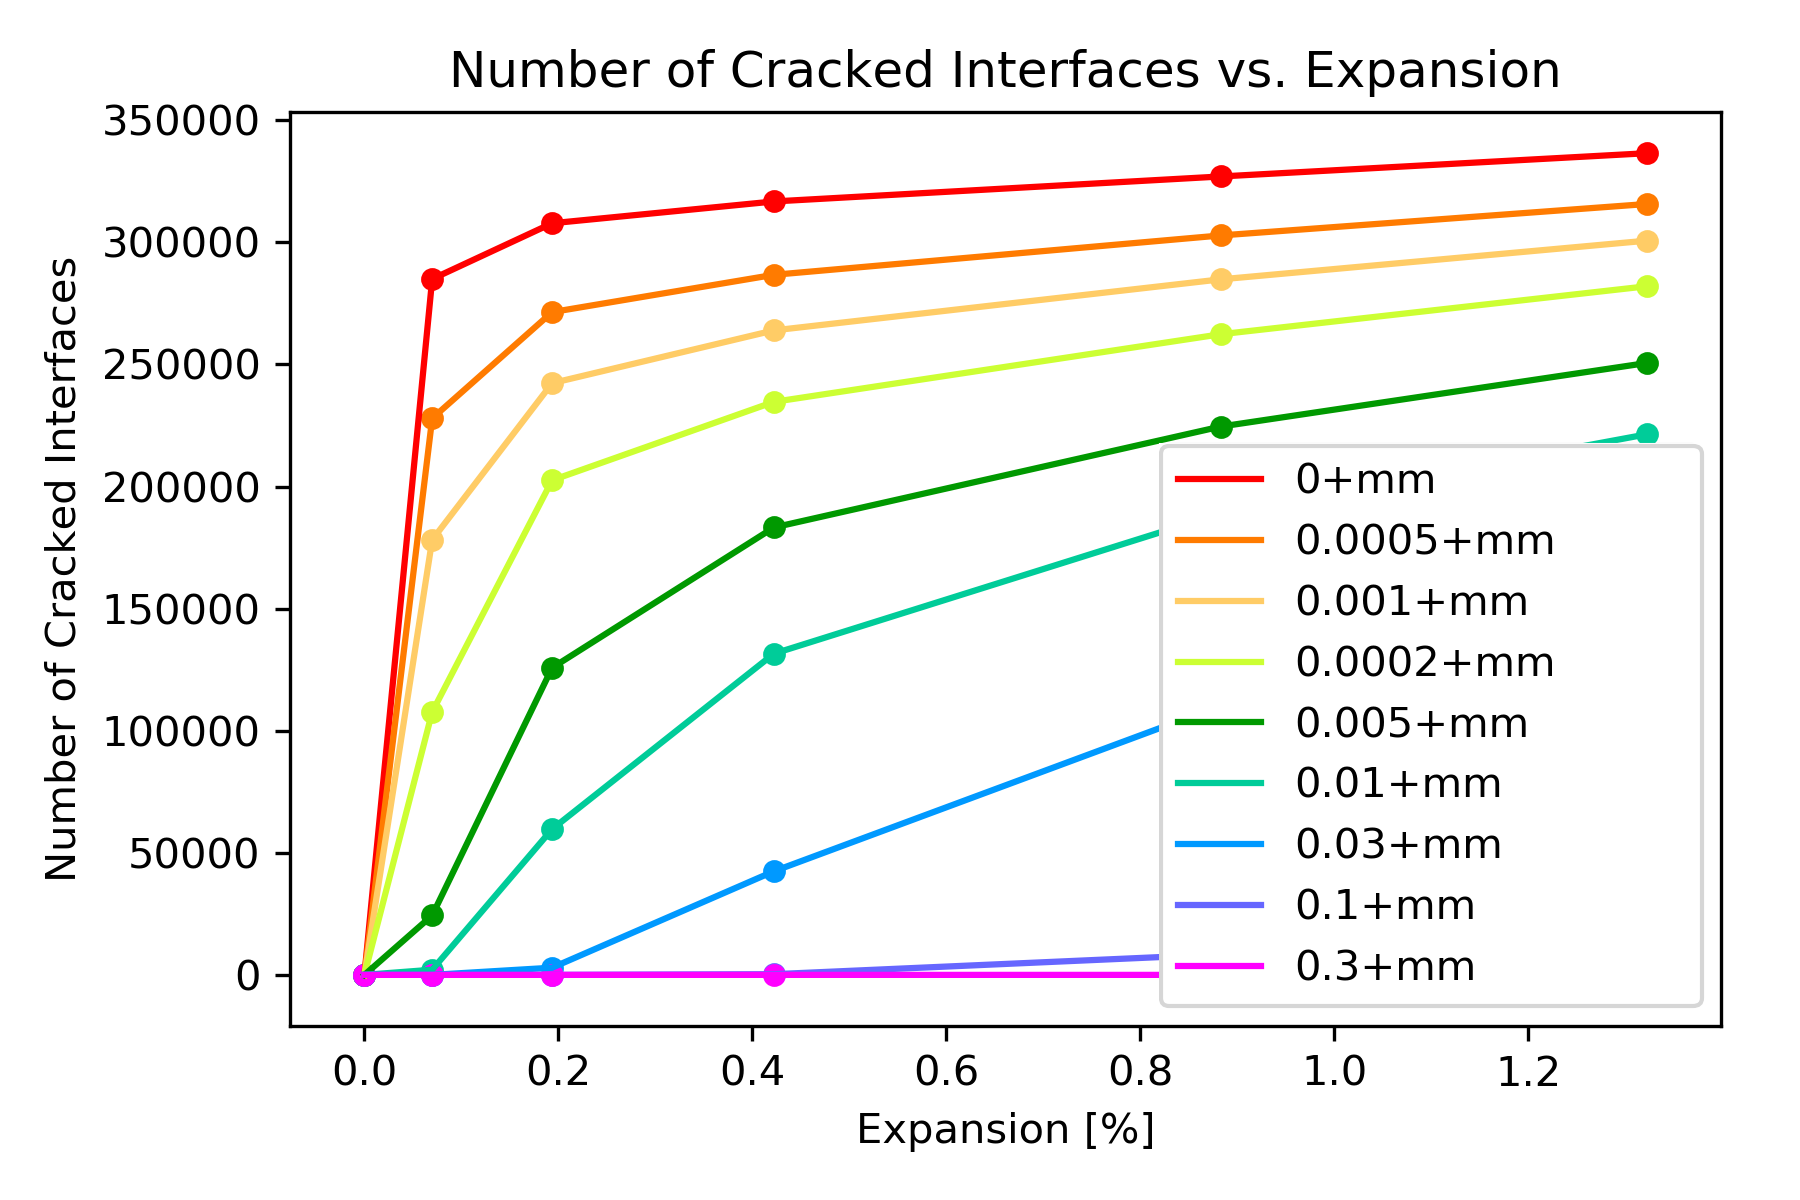
\includegraphics[width=.8\linewidth]{Files/interface/A30P75CRACK.png}
  \caption{Number of Cracked Interface vs. Expansion}
  \label{A30P75CRACKkk}
\end{figure}
